\documentclass[border=4pt]{standalone}
\usepackage[utf8]{inputenc}
\usepackage[T1]{fontenc}
\usepackage{lmodern}
\usepackage{amsmath,amssymb,mathtools}
\usepackage{tikz}
\usetikzlibrary{calc,decorations.pathreplacing,angles,quotes}
\usepackage{pgfplots}
\pgfplotsset{compat=1.18}
% Figura extraída de la Tarea 11 de Cálculo I (primer semestre).
\begin{document}
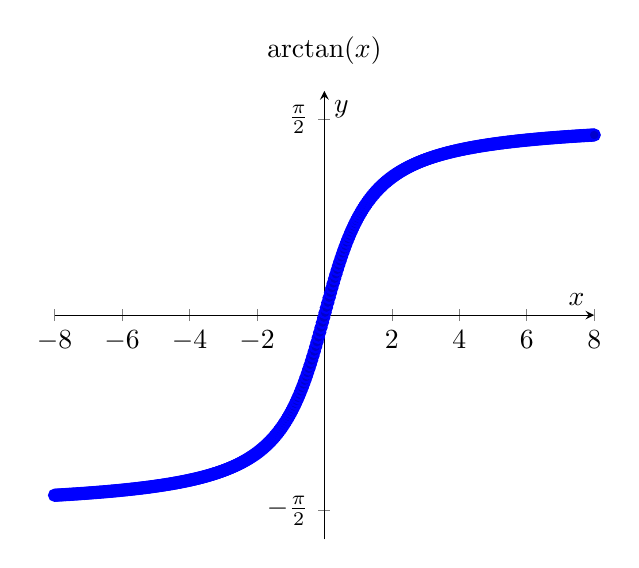
\begin{tikzpicture}
        \begin{axis}[
        domain=-8:8,samples=400,
        xmin=-8,xmax=8,ymin=-1.8,ymax=1.8,
        axis lines=middle,xlabel={$x$},ylabel={$y$},
        ytick={-1.5708,0,1.5708},
        yticklabels={\(-\tfrac{\pi}{2}\),0,\(\tfrac{\pi}{2}\)},
        title={\(\operatorname{arctan}(x)\)}
        ]
        \addplot+[thick]{atan(x)*pi/180};
        \end{axis}
    \end{tikzpicture}
\end{document}
